\documentclass[a4paper, 12pt]{article}
\usepackage{amsmath}
\usepackage{amsfonts, amsthm, amssymb} % this has the proof environment
\usepackage[top=1in, bottom=1in, left=.8in, right=.8in]{geometry} % good margins

% images 
\usepackage{graphicx}
\graphicspath{ {./images/} }

%verilog code
\usepackage{xcolor}
\usepackage{listings}
\definecolor{vgreen}{RGB}{104,180,104}
\definecolor{vblue}{RGB}{49,49,255}
\definecolor{vorange}{RGB}{255,143,102}

\lstdefinestyle{verilog-style}
{
    language=Verilog,
    basicstyle=\small\ttfamily,
    keywordstyle=\color{vblue},
    identifierstyle=\color{black},
    commentstyle=\color{vgreen},
    numbers=left,
    numberstyle=\tiny\color{black},
    numbersep=10pt,
    tabsize=8,
    moredelim=*[s][\colorIndex]{[}{]},
    literate=*{:}{:}1
}

\makeatletter
\newcommand*\@lbracket{[}
\newcommand*\@rbracket{]}
\newcommand*\@colon{:}
\newcommand*\colorIndex{%
    \edef\@temp{\the\lst@token}%
    \ifx\@temp\@lbracket \color{black}%
    \else\ifx\@temp\@rbracket \color{black}%
    \else\ifx\@temp\@colon \color{black}%
    \else \color{vorange}%
    \fi\fi\fi
}
\makeatother

\usepackage{trace}

\newcommand{\paren}[1]{\left(#1\right )}
\newcommand{\set}[1]{\left \{#1\right \}}
\newcommand{\R}[0]{\mathbb R}
\newcommand{\Z}[0]{\mathbb Z}
\newcommand{\de}[0]{\text{\normalfont d}}
\newcommand{\mycomment}[1]{}


\begin{document}

\title{\vspace*{-.9in}Lab 1: Iterative Multiplier / Divider}
\date{Due: 2/3/2023}
\author{Michael Tu}
\maketitle
\hrule

\section{Abstract}
The purpose of this lab was to implement the multiplication and division modules of a combined multiplication / division unit capable of performing several types of signed and unsigned operations. The lab served to familiarize students with verilog as well as control-datapath design principles and the val-rdy interface scheme. 

\section{Design}
My design for this lab followed the datapath presented almost exactly. I modularized heavily and used many of the modules provided in the \texttt{vc} folder.

\subsection{Control Unit}
For both the iterative multiplication and division units, my control unit implemented a state machine with three states: WAIT, CALC, and DONE. Transitions happened according to the following state machine diagram
\begin{center}
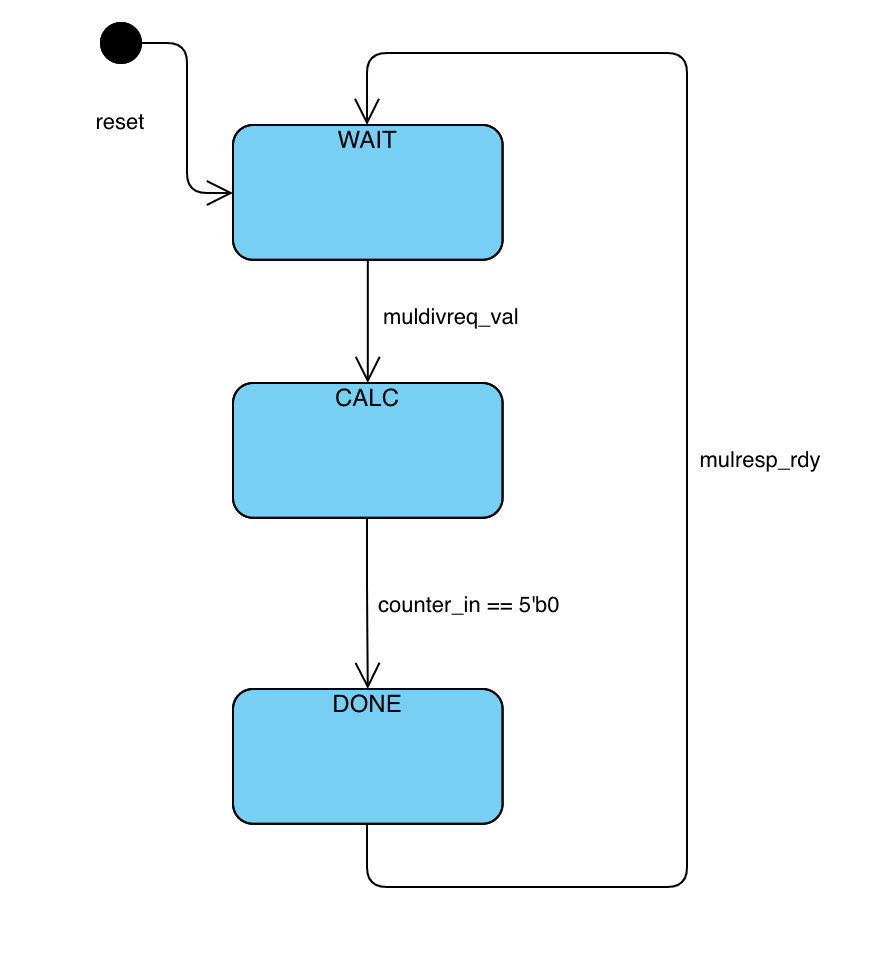
\includegraphics[scale=.5]{state-machine}
\end{center}
My machine entered the WAIT state when it was ready to accept new inputs, computed the results of the algorithm in the CALC state, and transmitted the final results in the DONE state. Both the WAIT and DONE states prevented calculation from occurring by disabling the counter in the datapath module.

Although not shown in the diagram, this was a mealy machine, and the control signals depended on values stored in registers in the datapath. Below is an example of the control signals output by the \texttt{DivIterative} unit.

\begin{lstlisting}[style={verilog-style}]
  case ( state )
      WAIT : begin
        divreq_rdy = 1'b1;
        cntr_mux_sel_out = 1'b1;
        		.
        		.
        		.
      end

      CALC : begin
        		.
        		.
        		.
        if (diff_sign_in)
          sub_mux_sel_out = 1'b0;
        else
          sub_mux_sel_out = 1'b1;

        divresp_val = 1'b0;
      end

      DONE : begin
        divreq_rdy = 1'b0;
        cntr_mux_sel_out = 1'b1;
        fn_sign_reg_en_out = 1'b0;
        sign_en_out = 1'b0;
        a_en_out = 1'b0;
        b_en_out = 1'b0;
        fn_sign_reg_en_out = 1'b1;

        if (rem_sign_in && fn_sign_in)
          rem_sign_mux_sel_out = 1'b0;
        else
          rem_sign_mux_sel_out = 1'b1;

        if (div_sign_in && fn_sign_in)
          div_sign_mux_sel_out = 1'b0;
        else
          div_sign_mux_sel_out = 1'b1;

        divresp_val = 1'b1;
      end
    endcase
    if (fn_sign_in)
      is_op_signed_out = 1'b1;
    else
      is_op_signed_out = 1'b0;
  end
\end{lstlisting}

In hindsight, it probably wasn't necessary to pass every single signal back through to the control unit, but it did allow for a clean separation of datapath and control which I appreciated. 

\subsection{Design Changes}
One design change that I added was a register for storing the value of the \texttt{divreq\_msg\_fn} since I discovered during some later testing that if the current \texttt{muldiv\_msg} and upcoming message had different signed-ness my code would use the signedness of the upcoming calculation when selecting the final output. This also required adding an extra control signal between the datapath and control modules.

\section{Testing}
For the most part, I kept my tests in the \texttt{IntMulDivIterative.t.v} file.

\subsection{Multiplier tests}
For my personal multiplier tests, I added three test cases where the result was longer than 32 bits. I split these up by signedness i.e., positive/positive, positive/negative, and negative/negative.

\subsection{Divider Tests}
For my divider tests, I added three tests of basic functionality: dividing with remainder and without remainder. I also added several signed tests where the divisor, dividend, or both inputs were meant to be interpreted as signed or unsigned.

\subsection{Combined Tests}
My combined tests were mainly about switching between different types of operations, ie signed/unsigned or multiplication/division.


\section{Evaluation}
The results of the test input were as follows:

\begin{center}
\begin{tabular}{ |p{3cm}|p{3cm}|p{3cm}|p{4.5cm}|p{1.5cm}|  }
 \hline
 \multicolumn{5}{|c|}{Test Results} \\
 \hline
 Operation & Input A & Input B & Output & Cycles\\
 \hline
 \hline
 mul & 0xdeadbeef & 0x10000000 & 0xfdeadbeef0000000 & 33\\
 div & 0xf5fe4fbc & 0x00004eb6 & 0xfffcdfee & 33\\
 rem & 0x0a01b044 & 0xffffb14a & 0x0a01b044 & 33\\
 divu & 0xf5fe4fbc & 0x00004eb6 & 0x00032012 & 33\\
 remu & 0x0a01b044 & 0x00004eb6 & 0x0a01b044 & 33\\
 \hline
\end{tabular}
\end{center}
\end{document}
